% \documentclass[letterpaper]{article}
\documentclass[journal]{IEEEtran}

\usepackage[margin=2.2cm]{geometry}
\usepackage[spanish,es-nodecimaldot]{babel}
\usepackage[utf8]{inputenc}
\usepackage[T1]{fontenc}
\usepackage{graphicx}
\usepackage{grffile}
\usepackage{longtable}
\usepackage{wrapfig}
\usepackage{rotating}
\usepackage[normalem]{ulem}
\usepackage{amsmath}
\usepackage{textcomp}
\usepackage{amssymb}
\usepackage{capt-of}
\usepackage{hyperref}
\usepackage{minted}
\usepackage{subfiles}
\usepackage[acronym, toc]{glossaries}

\usepackage{fancyhdr}
\usepackage{graphicx}
\usepackage{xcolor}
\usepackage{multicol}

\usepackage{grffile}
\usepackage{longtable}
\usepackage{wrapfig}
\usepackage{rotating}
\usepackage[normalem]{ulem}
\usepackage{amsmath}
\usepackage{textcomp}
\usepackage{amssymb}
\usepackage{capt-of}
\usepackage{hyperref}

\definecolor{LightGray}{gray}{0.9}
\definecolor{DarkGray}{gray}{0.1}
\definecolor{Base03}{HTML}{f8f8f8}

\usemintedstyle{emacs}



\renewcommand{\listingscaption}{Script}
\renewcommand\listoflistingscaption{Índice de \listingscaption\@'s}
\setminted[bash]{frame=lines,framesep=2mm,baselinestretch=1.2,fontsize=\scriptsize,breaklines=true,bgcolor=Base03}
\setminted[bat]{frame=lines,framesep=2mm,baselinestretch=1.2,fontsize=\scriptsize,breaklines=true,bgcolor=Base03}
\setminted[linux-config]{frame=lines,framesep=2mm,baselinestretch=1.2,fontsize=\scriptsize,breaklines=true,bgcolor=Base03}
\setminted[shell-session]{frame=lines,framesep=2mm,baselinestretch=1.2,fontsize=\scriptsize,breaklines=true,bgcolor=Base03}
\graphicspath{{./img_common}{../images}}
% \pagestyle{fancy}
% \fancyfoot[R]{\thepage}
% \fancyfoot[C]{
\includegraphics[width=0.1\textwidth]{inge_logo}}
% \fancyhead[L]{\leftmark}
% \fancyhead[R]{\rightmark}

\hypersetup{
 pdfauthor={Gonzalez Gonzalez Claudio, Mansur Jiménez Arturo, Romero Andrade Cristian, Romero Andrade Vicente},
 pdftitle={Proyecto SD},
 pdfkeywords={},
 pdfsubject={},
 pdfcreator={LuaTex},
 pdflang={Spanish}}

\title{Proyecto: Implementación de un servidor con sincronización usando NIS-SAMBA-Active Directory}

\author{
  \IEEEauthorblockN{Gonzalez Gonzalez Claudio,
  Mansur Jiménez Arturo,
    Romero Andrade Cristian,
    Romero Andrade Vicente}
  \IEEEauthorblockA{Sistemas Distribuidos\\
Facultad de Ingeniería\\
Universidad Nacional Autónoma de México\\
}}
\newcommand\indexspace{\par \vskip 15\p@ \@plus5\p@ \@minus3\p@\relax}
\usepackage{microtype}



\newglossaryentry{SAMBA}
{
  name=SAMBA,
  description={Es una implementación libre del protocolo de archivos
    compartidos de Microsoft Windows para sistemas de tipo UNIX}
}
\newglossaryentry{ldap}
{
  name=LDAP,
  description={El protocolo ligero de acceso a directorios hace referencia a un
    protocolo a nivel de aplicación que permite el acceso a un servicio de
    directorio ordenado y distribuido para buscar diversa información en un
    entorno de red}
}

\newglossaryentry{kerberos}
{
  name=Kerberos,
  description={Es un protocolo de autenticación de redes de ordenador creado
    por el MIT que permite a dos ordenadores en una red insegura demostrar
    su identidad mutuamente de manera segura}
}

\newglossaryentry{nfs}
{
  name=NFS,
  description={Network File System es un
    protocolo de nivel de aplicación, según el Modelo OSI.~Es utilizado para
    sistemas de archivos distribuido en un entorno de red de computadoras de
    área local. Posibilita que distintos sistemas conectados a una misma red
    accedan a ficheros remotos}
}

\newglossaryentry{autofs}
{
  name=AutoFS,
  description={Es un servicio por parte del cliente que monta
    automáticamente el sistema de archivos adecuado.}
}

\newglossaryentry{fstab}
{
  name=fstab,
  description={Es un fichero que se encuentra comúnmente en
    sistemas Unix (en el directorio \texttt{/etc/}) como parte de la
    configuración del sistema. Lo más destacado de este fichero es la lista de
    discos y particiones disponibles. En ella se indica como montar cada
    dispositivo y qué configuración utilizar}
}

\newglossaryentry{systemd}
{
  name=systemd,
  description={Es un conjunto de demonios o daemons de
    administración de sistema, bibliotecas y herramientas diseñados como una
    plataforma de administración y configuración central para interactuar con
    el núcleo del Sistema operativo GNU/Linux.}
}






\newacronym{ntp}{NTP}{Network Time Protocol}
\newacronym{nfs}{NFS}{Network File System}
\newacronym{nis}{NIS}{Network Information Service}
\newacronym{smb}{SMB}{Server Message Block}

\makeglossaries{}

\begin{document}

\markboth{04 de febrero de 2020}

\begin{titlepage}
  \centering{
    
\includegraphics[width=0.3\textwidth]{unam_logo}\vfill{}
    {\scshape{\Huge Facultad de Ingeniería\par{}}}\vspace{0.5cm}
    {\scshape{\Large Sistemas Distribuidos\par{}}}\vfill{}
    {\huge \textbf{Proyecto}}\vfill{}

    {\Large
      Alumnos
      \begin{itemize}
        \item Gonzalez Gonzalez Claudio
        \item Mansur Jiménez Arturo
        \item Romero Andrade Cristian
        \item Romero Andrade Vicente
      \end{itemize}
      % \textbf{Equipo  }

    }\vfill{}
    {\large Profesor: ING.~Guadalupe Lizeth Parrales Romay}\vfill{}
    
\includegraphics[width=0.1\textwidth]{inge_logo}
  }
\end{titlepage}




\twocolumn[
\begin{@twocolumnfalse}
\tableofcontents
\end{@twocolumnfalse}
\bigskip{}]





\twocolumn[
\begin{@twocolumnfalse}
\maketitle
\begin{abstract}
  En el presente trabajo se implementa la sincronización de cuentas así como
  sus claves a través de una red de área local a distintas máquinas de
  distintos sistemas operativos.
\end{abstract}

\section{Introducción}\label{sec:introduccion}
En la presente se describe una serie de pasos para llevar a cabo la
administración central de usuarios a un servidor basado en Linux. Existen
varias herramientas para llevar a cabo esta tarea, para compartir archivos se
utilizó \Gls{SAMBA} y \Gls{NIS} para montar los archivos del servidor a varios
ordenadores conectados al servidor maestro. Para la autenticación se optó
Active Directory y \Gls{kerberos} para tener compatibilidad tanto con sistemas
basados en Linux y Windows.

Estas herramientas son útiles ya que permiten a los hosts, independientemente
su sistema operativo, autenticarse a un servidor basado en Linux. Es es
una opción excelente en un entorno T.I. (tecnología de la información)
heterogéneo con distintos sistemas operativos.
\end{@twocolumnfalse}
\bigskip{}]

\section{Arquitectura}\label{sec:arq}
\begin{figure}[h!]
  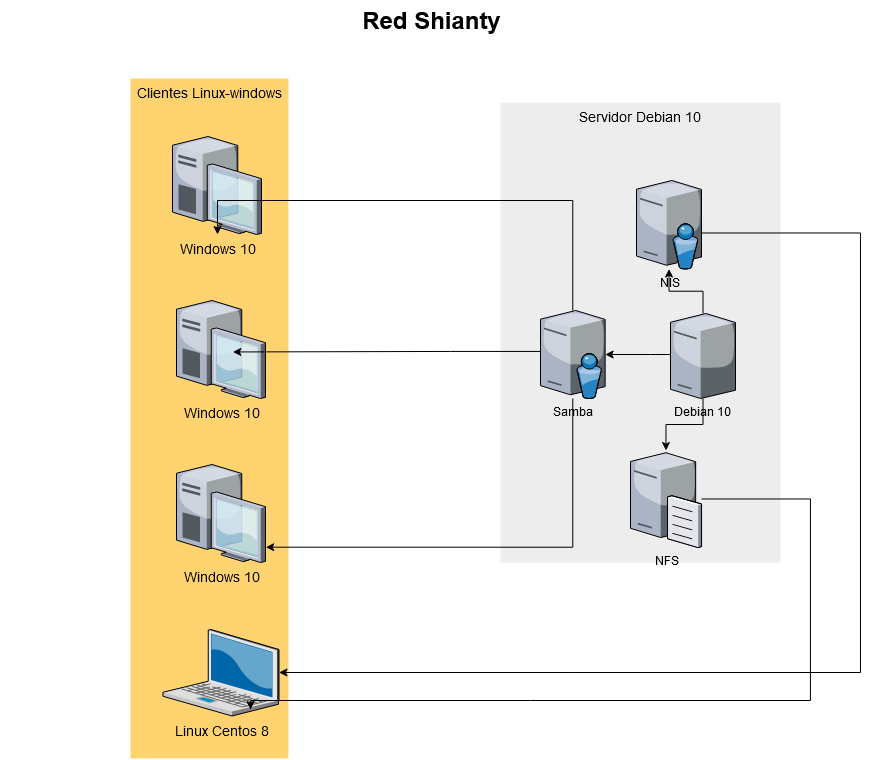
\includegraphics[width=0.5\textwidth]{arquitectura}
  \caption{Arquitectura de la red}\label{fig:arquitectura}
\end{figure}
\begin{figure}[h!]
  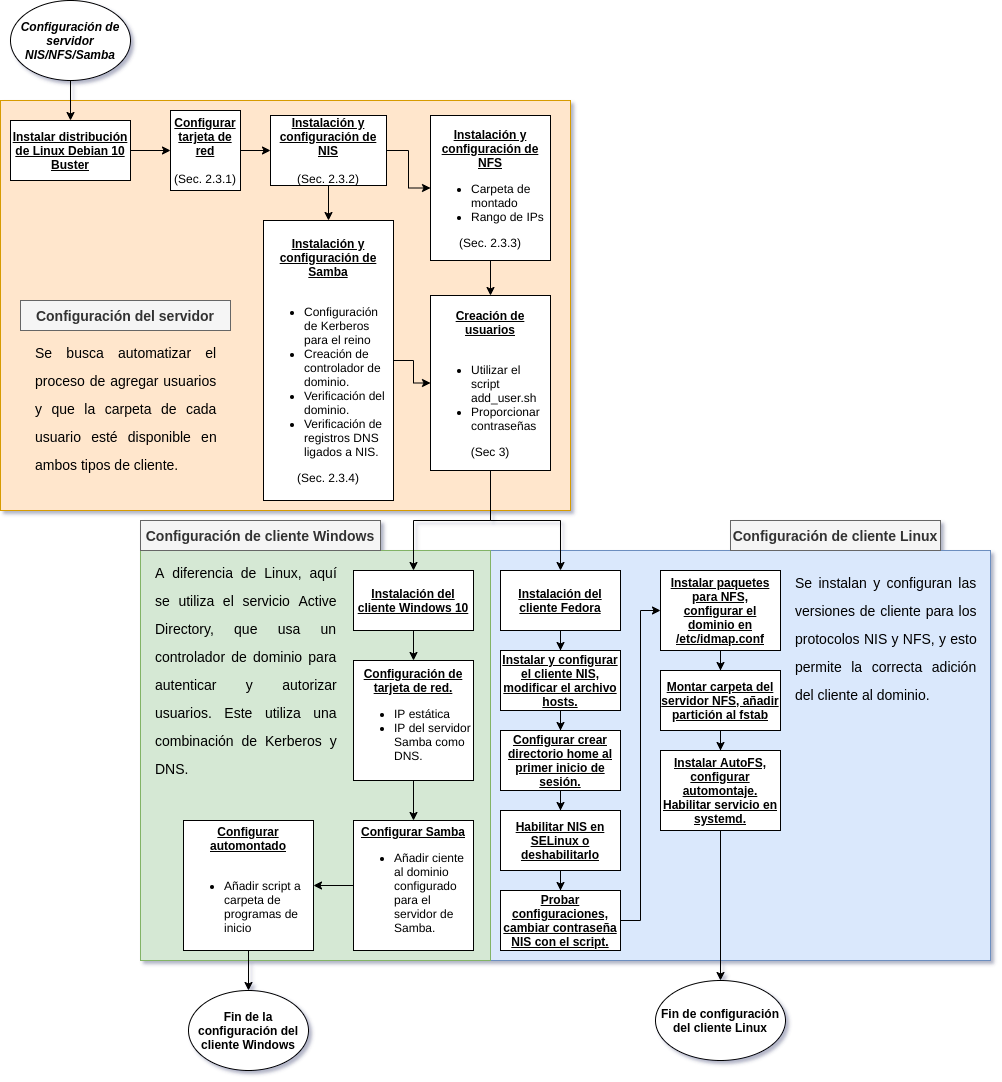
\includegraphics[width=0.5\textwidth]{Diagrama_Shianty}
  \caption{Diagrama cliente-servidor}\label{fig:dia_c_s}
\end{figure}

\cleardoublepage{}

\section{Recursos}\label{sec:recursos}

\subfile{contenido/material_utilizado.tex}

\cleardoublepage{}

\section{Creación de Usuarios}\label{sec:cusuarios}

\subfile{contenido/usuarios.tex}

\cleardoublepage{}

\section{Clientes}\label{sec:clientes}

\subfile{contenido/cliente.tex}
\newpage{}
\section{Conclusión}\label{sec:conclusion}
Se utilizaron distintos protocolos para llevar a cabo la distribución
de los archivos de los usuarios que se crean en el servidor
maestro (\ref{sec:nis}), también en casos se implemento una manera para
volver a reactivar la conexión servidor (para Linux) en caso de
que este se encuentre
desconectado por factores externos, esta esta descrita en la
sección~\ref{sec:cliente_linux}.
El uso de los protocolos descritos en el \hyperref[glo:glosario]{glosario}
nos ayuda a crear nuestra red de usuarios sin tener que crear uno por uno
en cada ordenador, al igual la persistencia de los datos de los usuarios cuando
ellos cambian de ordenador, ya que gracias \Gls{SAMBA}, el directorio
\texttt{/home} del usuario se monta en cada PC donde, para acceder a esta
carpeta, debe ser el mismo usuario con su cuenta usando protocolos de
autenticación como Active Directory.


\vfill{}

\addcontentsline{toc}{section}{Índice de figuras}
\listoffigures
\addcontentsline{toc}{section}{Índice de códigos}
\listoflistings{}
\printglossary{}\label{glo:glosario}
\printglossary[type=\acronymtype]

\end{document}
